%------------------------------------------------------------------
% Preamble: provides useful commands and default settings
%------------------------------------------------------------------
%==================================================
% Standard
%==================================================
\documentclass[11pt]{article} % Page setup
\usepackage[top=1in, bottom=1in, left=1in, right=1in]{geometry} % Margin setup
\usepackage[square,sort,comma,numbers]{natbib}  % Reference Formatting
\usepackage{fancyhdr} % Header setup
\usepackage[toc,page]{appendix}
\usepackage[hang,flushmargin]{footmisc}
\usepackage{textpos}

%==================================================
%Typesetting Packages
%==================================================
\usepackage[colorlinks=true,linkcolor=Blue,citecolor=Red,urlcolor=Blue]{hyperref} % sets the color of hyperlinks
\usepackage{url} %Allows urls to be displayed properly
\usepackage{amsmath,amssymb} % Highly recommended as an adjunct to serious mathematical typesetting; amssymb provides extended symbol collection
\usepackage{textcomp} % Package supports Text Companion fonts (baht, bullet, copyright, musicalnote, onequarter, section, and yen)
\usepackage{color} % Provides foreground (text, rules, etc.) and background color management
\usepackage{colordvi} % Allows for using named colors when typsetting output
\usepackage[usenames,dvipsnames,svgnames,table]{xcolor} % Extends the color package; several color tints, shades, tones, and mixes of arbitrary colors
\definecolor{arsenic}{rgb}{0.23, 0.27, 0.29}
\definecolor{color18}{rgb}{0.5,0.5,0.5} % Defines a color named "color18"
\usepackage{bm} % bold math
\usepackage{siunitx} % si units package 
\newcommand{\SIper}{\SI[per-mode=symbol]} % Special command for the SI unit package
\usepackage{enumerate} % Allows for the enumerate style to be changed 
%\usepackage{enumitem}
\usepackage{alphalph}
\usepackage{setspace}
\usepackage{blindtext}
\usepackage{soul}
\usepackage[tocindentauto]{tocstyle}
\usepackage{algorithm}
\usepackage{algpseudocode}
\usepackage{multirow}
\usepackage{mathtools}
\usepackage{minted}
\usepackage{afterpage}
\usepackage{float}
\usepackage{changepage}
\numberwithin{equation}{section}
%\usepackage{mathptmx}

% ==================================================
%Figure packages
% ==================================================
\usepackage{graphicx} % Include figure files
\usepackage{rotating} % Performs all rotations including complete figures and tables with their captions ON ONE PAGE
\usepackage{lscape} % Rotates the page contents but not the page number; can be applied across many pages
\usepackage[font=scriptsize,format=plain,labelfont=bf]{caption} % Caption customization (also for tables)
\usepackage{subcaption} % Provides support for subcaptions
\usepackage{float} % Improved interface for defining float objects (figures and tables)
\usepackage{wrapfig} % Allows figures or tables to have text wrapped around them
\setlength{\parskip}{5pt} %Space between paragraphs
\setlength{\parindent}{0pt} %Paragraph Indent size
\usepackage{fancybox}
\usepackage{mdframed}
\usepackage{makeidx}
\usepackage{tablefootnote}

% ==================================================
% Table packages
% ==================================================
\usepackage{longtable} % allow multipage tables
\usepackage{multicol}
\usepackage{multirow} % create tabular cells spanning multiple rows
\usepackage{dcolumn} % Align table columns on decimal point
\usepackage{threeparttable}
\usepackage{lipsum,booktabs}

% ==================================================
% Section Formatting 
% ==================================================
\usepackage{sectsty}
\allsectionsfont{\bfseries} %Sets ALL section font

%Title, author, date formats	
	\newcommand{\mytitle}[1]{\title{\bf{\textsf{#1}}}}
	\newcommand{\myauthor}[1]{\author{\textsf{#1}}}
	\newcommand{\mydate}[1]{\textsf{\date{#1}}}
	\newcommand{\mytoday}{\textsf{\today}}

%Section header formats	(Numbered)
	\newcommand{\mysection}[2]{\vspace{-5px}\section{#1}\label{#2}\vspace{-10px}}
	\newcommand{\myssection}[2]{\vspace{-5px}\subsection{#1}\label{#2}\vspace{-5px}}
	\newcommand{\mysssection}[2]{\vspace{-5px}\subsubsection{#1}\label{#2}\vspace{-5px}}

%Section header formats	(Unnumbered)	
	\newcommand{\mysectionN}[2]{\vspace{-5px}\section*{#1}\label{#2}\vspace{-10px}}
	\newcommand{\mysectionnonum}[2]{\vspace{-5px}\section*{#1}\label{#2}\vspace{-10px}}
	\newcommand{\myssectionN}[2]{\vspace{-5px}\subsection*{#1}\label{#2}\vspace{-5px}}
	\newcommand{\myssectionnonum}[2]{\vspace{-5px}\subsection*{#1}\label{#2}\vspace{-5px}}
	\newcommand{\mysssectionN}[2]{\vspace{-5px}\subsubsection*{#1}\label{#2}\vspace{-5px}}
	\newcommand{\mysssectionnonum}[2]{\vspace{-5px}\subsubsection*{#1}\label{#2}\vspace{-5px}}

%Paragraph header formats		
	\newcommand{\mypart}[2]{\part{#1}}
	\newcommand{\mypara}[2]{\paragraph{#1}}
	\newcommand{\myparaN}[2]{\paragraph*{#1}}
	\newcommand{\myparanonum}[2]{\paragraph*{#1}}

%References, etc.	
	\newcommand{\myref}[2]{\hyperref[#2]{#1~\ref{#2}}}
	\newcommand{\myrefexp}[3]{\hyperref[#3]{{#1}~{#2}}}
	\newcommand{\hilight}[1]{\colorbox{yellow}{#1}}
	\newcommand{\myfilename}[1]{\texttt{\textsf{#1}}}
	\newcommand{\mywebsite}[1]{\myfilename{\bf #1}}
	\newcommand{\commandline}[1]{\texttt{> #1}}
	\newcommand{\plusplus}[1]{#1{}\texttt{++}}

%Callout Box Creator	
	\newcommand{\callout}[3]
	{
	\begin{wrapfigure}{#1}{#2\textwidth}
	\vspace{-20pt}
	\centering
	\fbox{\parbox{#2\textwidth}{#3}}
	\vspace{-10pt}
	\end{wrapfigure}
	}

% ==================================================
% Track changes and commenting packages/commands
% ==================================================
\usepackage{todonotes}
	\newcommand{\sn}[1]{\todo[color=magenta!40,caption={}]{#1}}
	
\usepackage{comment}


	%Other colors available 
	%cyan
	%green
	%white
	%darkgray
	%brown
	%olive
	%pink
	%purple
	%violet


\usepackage{verbatimbox}
\usepackage{wrapfig} 
\usepackage{rotating}
\usepackage{mathrsfs}
\usepackage{cancel}
\usepackage{pdfpages}
\newcommand{\bs}{\boldsymbol}
\newcommand{\kpar}{k_{\shortparallel}}
\newcommand{\chebint}{\pmb{\mathscr{I}}}
\newcommand{\chebdiff}{\pmb{\mathscr{D}}}
\newcommand{\overbar}[1]{\mkern 1.5mu\overline{\mkern-1.5mu#1\mkern-1.5mu}\mkern 1.5mu}

%---------
% Beginning of document
%------------------------------------------------------------------
\begin{document}
\setcounter{secnumdepth}{5}
\setcounter{tocdepth}{4}
% Your Name
\begin{textblock*}{8cm}(15cm,-1cm)
	\noindent {Sachin Natesh} 
\end{textblock*}

\mysection{Stokes flow}{}
This repository concerns the solution of Stokes equations,
\begin{align}
\displaystyle \eta \nabla^2 \bs u - \nabla p &= -\bs f, \label{momentum}\\
\nabla \cdot \bs u &= 0, \label{continuity}
\end{align}
on some domain $\Omega := (x,y,z) \in[0,L_x] \times [0,L_y] \times [0,L_z]$ subject to some boundary conditions (BCs). Here, the velocity $\bs u = \begin{pmatrix}u & v & w \end{pmatrix}^T$, and $\bs f = \begin{pmatrix}f & g & h \end{pmatrix}^T$ are smeared $\delta$-function sources representing particles with an effective hydrodynamic radius of $R_h$. The boundary conditions, imposed on the faces of $\Omega$, can be combinations of \texttt{open}, \texttt{periodic}, \texttt{mirror wall} or \texttt{inverse mirror wall}. The latter two correspond to a confined geometry, and some BC must be prescribed at both endpoints of each axis.

The source term $\bs f$ consists of monopole and dipole terms with ``exponential of a semicircle" (ES) kernel \cite{barnett} envelopes $\Delta$;
\begin{equation}
\Delta(z;\alpha,\beta) = \displaystyle \frac{1}{\displaystyle \int_{-\alpha}^\alpha e^{\beta(\sqrt{1-(\frac{z}{\alpha})^2}-1)}dz} \begin{cases}
e^{\beta(\sqrt{1-(\frac{z}{\alpha})^2}-1)},\quad &|\frac{z}{\alpha}| \leq 1\\
0,\quad &\text{otherwise}.
\end{cases}
\end{equation}
Here, $\alpha = w_ih_i/2$, where $h_i$ is the grid spacing in direction $i$ ($x,y$ or $z$), $w_i$ is the number of points to which we spread in that direction, and we've normalized the kernel so that integrating it over its support gives 1. The monopole term $\Delta_f$ represents the force exerted by particles on the fluid, while the dipole term $\Delta_\tau$ relates to external torques $\bs \tau$ on the particles, given in \cite{lomholt} as
\begin{equation}\label{fcm}
\bs f(\bs x) = \displaystyle \sum_{k=1}^M \bs f(\bs y_k)\Delta_f(\bs x - \bs y_k) +\frac{1}{2}\nabla \times  \big(\bs{\tau}(\bs y_k)\Delta_\tau(\bs x - \bs y_k)\big) ,
\end{equation}
where $\bs y_k$ is the position of particle $k$. Once we've solved for the fluid velocity $\bs u$, we can obtain the linear and angular velocities of the particles through
\begin{align}
\bs V(\bs y_k) &= \displaystyle \int_\Omega \bs u(\bs x) \Delta_f(\bs x - \bs y_k)d\bs x,\label{getpartvels}\\
\bs \Omega(\bs y_k) &= \frac{1}{2}\displaystyle \int_\Omega \big(\nabla \times \bs u(\bs x)\big) \Delta_\tau(\bs x - \bs y_k)d\bs x\label{getpartvort}.
\end{align}

Note, the kernel parameters given above correspond to uniform grids. When the grid is not uniform in a given direction, we use the relation
\begin{equation}
\alpha = \frac{w R_h}{2 c_{f|\tau}(w)},
\end{equation}
where $w$ and $c_{f|\tau}(w)$ are the width and dimensionless radius (of monopole or dipole) of the ES kernel found in tables listed in the report deriving the DP-wall solver (ADD HERE).
\mysection{Describe the SpreadInterp library}{}
\myssection{How to handle various BCs}{}
\mysection{Describe the Python interface}{}
\myssection{A note on memory layout}{}
Data on the grid are stored so that the fastest index is $l = 0,\cdots,\texttt{dof}$, followed by $i = 0,\cdots,N_x$, then $j = 0, \cdots, N_y$, and with $k = 0,\cdots ,N_z$ the slowest. This means that the \texttt{Grid} member \texttt{fG} is such that \texttt{fG}(k,j,i,l) = \texttt{fG[l + dof * (i + Nx * (j + Ny * k))]}.
The reason for this has to do with parallelization and vectorization in the underlying spreading algorithm, where it's better if $x$ and $y$ vary faster than $z$. However, this isn't necessarily true for the solve stage. 

In the Python interface, when we execute 

\hspace{10pt} \texttt{fG = Spread(species, grid, Nx * Ny * Nz * dof)}, 

the returned variable \texttt{fG} has been marshalled into a flat \texttt{numpy} array. If it makes sense (based on the solver) to \emph{copy} the memory layout to a new one, say in reverse order, one can use

\hspace{10pt} \texttt{fG = np.transpose(np.reshape(fG, (Nz,Ny,Nx,dof)), (3,2,1,0)).copy()}

Then, the \texttt{fG} variable will be indexed in memory like \texttt{fG[l,i,j,k]} with $k$ the fastest index. Note, without the \texttt{copy()} operation appended at the end, we will only get a new \emph{view} of the memory layout, while the actual layout will remain unchanged.
\mysection{Triply periodic solver}{}
Suppose now that $\Omega$ is a triply periodic domain and we impose periodic boundary conditions on $\bs u$ and $p$. Taking the divergence of \myref{Eq.}{momentum} and using \myref{Eq.}{continuity}, we find the pressure $p$ satisfies a Poisson equation
\begin{equation}\label{poisson}
\nabla^2 p = -\nabla \cdot \bs{f}
\end{equation}
Then, taking the Fourier transform of \myref{Eq.}{poisson} and using Fourier derivative symbols, we find
\begin{equation}\label{psol}
\hat{p} = \displaystyle -\frac{i\bs{k} \cdot \hat{\bs f}}{k^2},
\end{equation}
where $\bs k = \begin{pmatrix} k_x & k_y & k_z\end{pmatrix}^T$ is the vector of wave numbers in $x, y$ and $z$, $k^2 = ||\bs k||^2$, and $\hat{\cdot}$ denotes the Fourier transform. Now, if take the Fourier transform of \myref{Eq.}{momentum} and use \myref{Eq.}{psol}, we find that
\begin{align}
\hat{u} &= \displaystyle \frac{1}{\eta k^2}\Big(\hat{f} + \frac{ik_x}{k^2}\big(ik_x \hat{f} + ik_y \hat{g} + ik_z \hat{h}\big)\Big),\\
\hat{v} &= \displaystyle \frac{1}{\eta k^2}\Big(\hat{g} + \frac{ik_y}{k^2}\big(ik_x \hat{f} + ik_y \hat{g} + ik_z \hat{h}\big)\Big),\\
\hat{w} &= \displaystyle \frac{1}{\eta k^2}\Big(\hat{h} + \frac{ik_z}{k^2}\big(ik_x \hat{f} + ik_y \hat{g} + ik_z \hat{h}\big)\Big).
\end{align}

The above equations hold for $k \neq 0$. Since the net force on the unit cell must be 0, we accept 0 as the solution for the $k=0$ mode of the fluid velocity.

In our uniform discretization, $k_i = \frac{2\pi j}{L_i}$, $j = -\frac{N_i}{2},\cdots, \frac{N_i}{2}-1$, with $N_i$ the number of points in direction $i=x,y,z$, and $L_i$ the length. 

\myssection{Validation (translation-only)}{}
Here, we will validate the efficacy of our method and implementation in computing particle velocities against Hasimoto's correction to Stokes drag law for cubic lattices of spheres \cite{hasimoto}, given by
\begin{equation}\label{pbccorr}
\displaystyle \frac{F}{\eta V} = \frac{6\pi R_h}{1 - 2.8373(R_h/L) + 4.19(R_h/L)^3 - 27.4(Rh/L)^6 + \text{h.o.t}},
\end{equation}
where $F$ is the force on the particle and $V$ is its velocity in one direction. We place a force of $\begin{pmatrix}1&0&0\end{pmatrix}$ on a particle of radius $R_h = 1.5539h$ located randomly in the unit cell $[0,L]^3$. This $R_h$ corresponds to ES kernel settings $w=6,\beta = 1.714 w$ with 0.02\% error from translational invariance. After spreading the force on the particle to the grid with the first term in \myref{Eq.}{fcm}, solving \myref{Eq.}{momentum} and interpolating the velocity on the particles with \myref{Eq.}{getpartvels}, we evaluate agreement with \myref{Eq.}{pbccorr}. The results, collected over several random placements of the particle and lattice lengths, are shown in the following figure.
\begin{figure}[H]
	\centering
	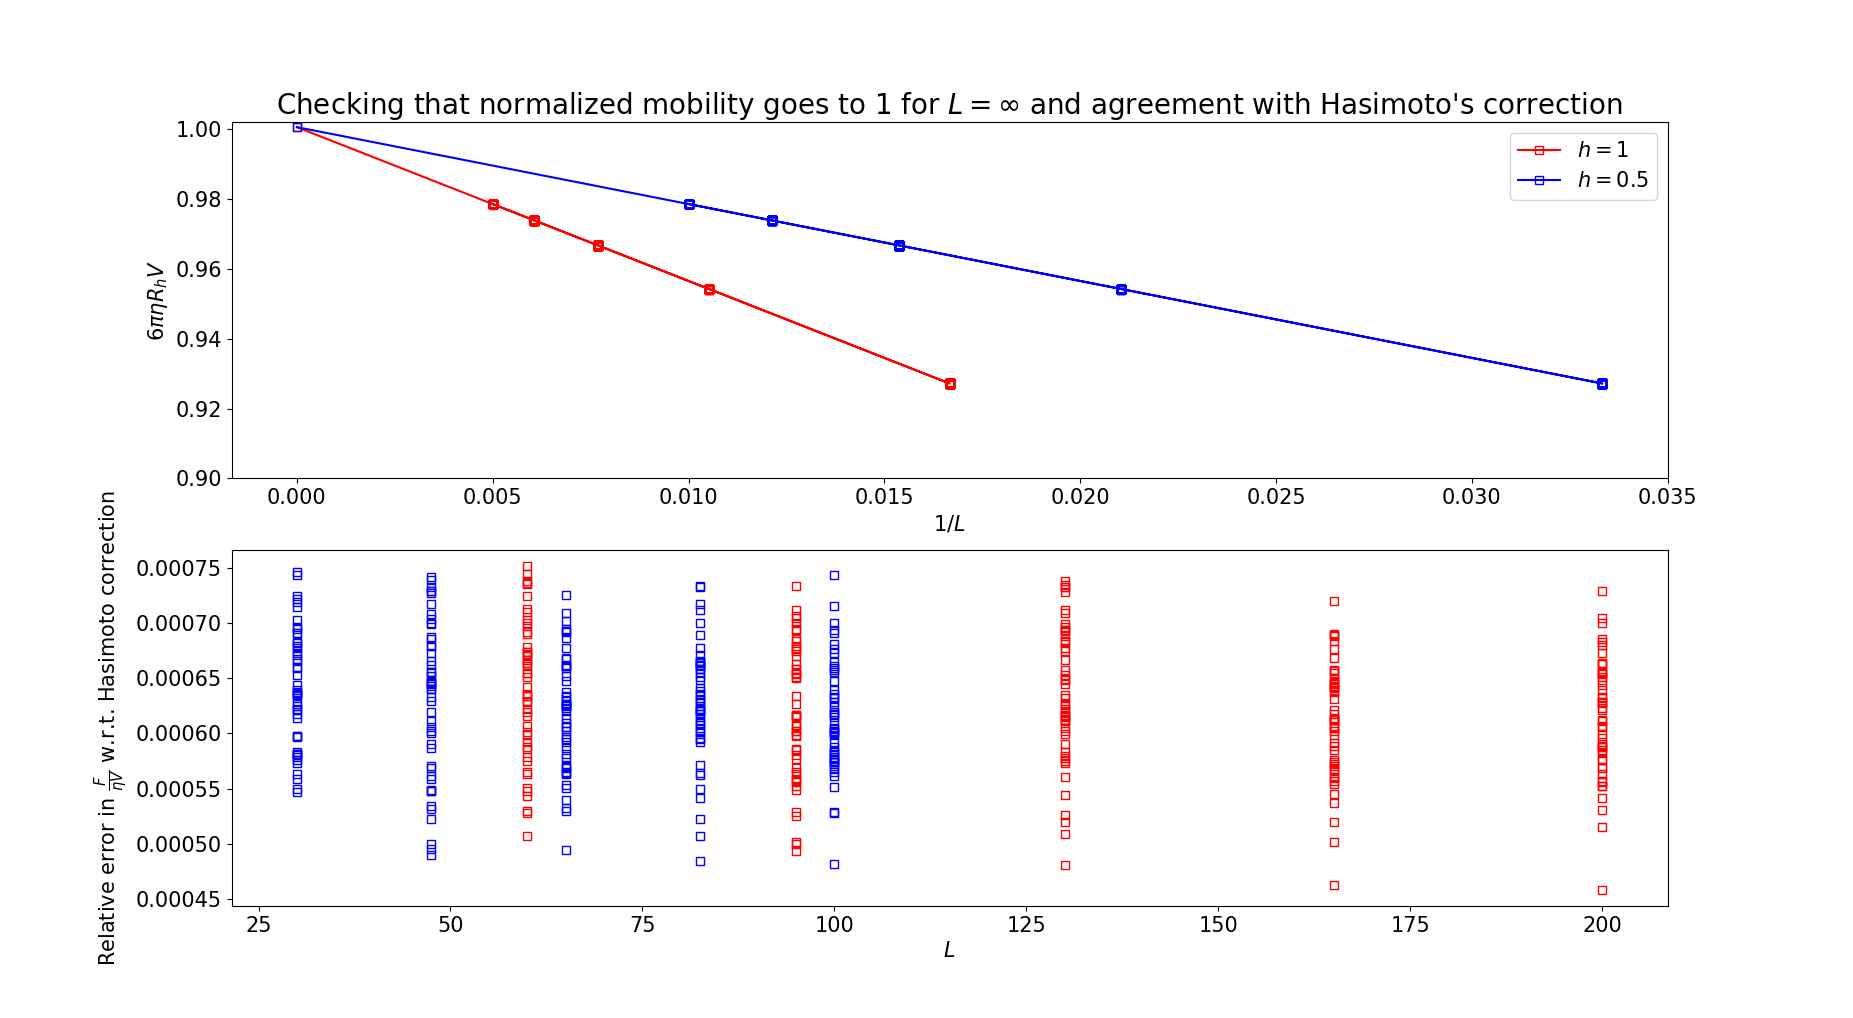
\includegraphics[width=1\linewidth]{./Figures/L_extrap_hasimoto_TP}
	\caption{In the top panel, we check that the normalized mobility extrapolates to approximately 1 for unit (blue) and non-unit (red) grid spacing $h$ as $L \to \infty$. The bottom figure assesses the relative agreement with Hasimoto's periodic correction to Stokes drag law \myref{Eq.}{pbccorr} for unit (blue) and non-unit (red) $h$. We achieve around 3 digits of accuracy, and the spread in the data corresponds well to the 0.02\% error due to loss in translational invariance of the ES kernel.}\label{fig4}
\end{figure}



\clearpage
\newpage
\addcontentsline{toc}{section}{References}
\bibliographystyle{unsrt}
%\bibliography{all_refs,NEMoSys,NEMoSys_extra,nemosysAV,autoverif_refs}
\bibliography{stokes_solver}
\end{document}
